\chapter{Introduction}
\label{ch1_intro}
\acg{[first draft - I have a lot of citations but other theses seem to not have many in the intro?]}

Humans have postulated that heat is a form of motion for a long time, but when the European Scientific Revolution led to the Age of Enlightenment in the 17th century, it became a subject of particularly ``heated'' debate~\cite{bacon_novum_1902,boyle_new_1660,halley_historical_1686,newton_vii_1997}. Scientists and philosophers also sought to explain diffusion, the general process by which something spreads out. As a result, in the 18th century, significant developments were made in understanding fluid mechanics and the kinetic theory of gases, as well as describing thermal conduction with similar frameworks~\cite{du_chatelet_dissertation_1744,bernoulli_hydrodynamica_1738,lomonosov_mikhail_1970}. With the birth of modern thermodynamics in the 19th century, scientists continued to make strides in understanding the motion of both heat and particles, from steam engines to fluids in motion~\cite{sadi_carnot_reflexions_1824,thomson_dynamical_1851,rudolf_clausius_mechanical_1867,fourier_analytical_1878,maxwell_theory_1908,joule_scientific_2011}. Of particular note were the Boltzmann transport equation, which characterized out-of-equilibrium thermodynamic systems through statistical quantities~\cite{boltzmann_weitere_1872}, and the Navier-Stokes continuum equations for fluid transport~\cite{navier_memoire_1827,stokes_effect_1851}. Experimental work during this time contributed to the understanding of diffusive processes -- Thomas Graham studied gas diffusion~\cite{graham_xxvii_1833} and Adolph Fick measured concentrations of salt in water, leading to the influential differential equations now referred to as Fick's laws of diffusion~\cite{fick_v_1855}.

\begin{figure*}[ht]
\begin{center}
\includegraphics[width=0.9\columnwidth]{Figures/randomwalk.png}
\caption{\label{fig:walk} A particle undergoing a one dimensional random walk. The particle begins at the origin (center), then through time, takes one ``step'' in a random direction after the other. \acg{[Placeholder until I find the old files for the next two figures on an ancient hard drive/recreate everything]}}
\end{center}
\end{figure*}

\begin{figure}[hb]
\begin{center}
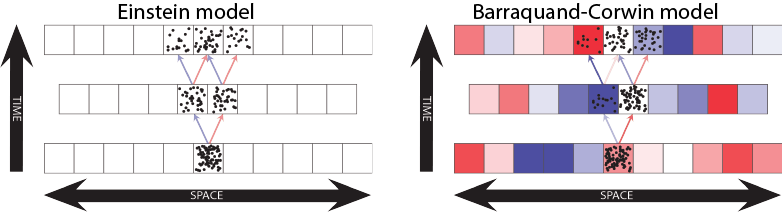
\includegraphics[width=0.9\columnwidth]{Figures/model_both_sidebyside.png}
\caption{\label{fig:1D_BC} 1D visualization of the Einstein and Barraquand-Corwin models, where the red and blue colors indicate the direction of each bias - right and left, respectively - and the color intensity indicates the strength of the bias; for example, a dark red square indicates a strong bias to the right for the particles inhabiting that square. White squares have an equal bias in each direction. Time increases from the bottom of the image toward the top.}
\end{center}
\end{figure}

\begin{figure*}[ht]
\begin{center}
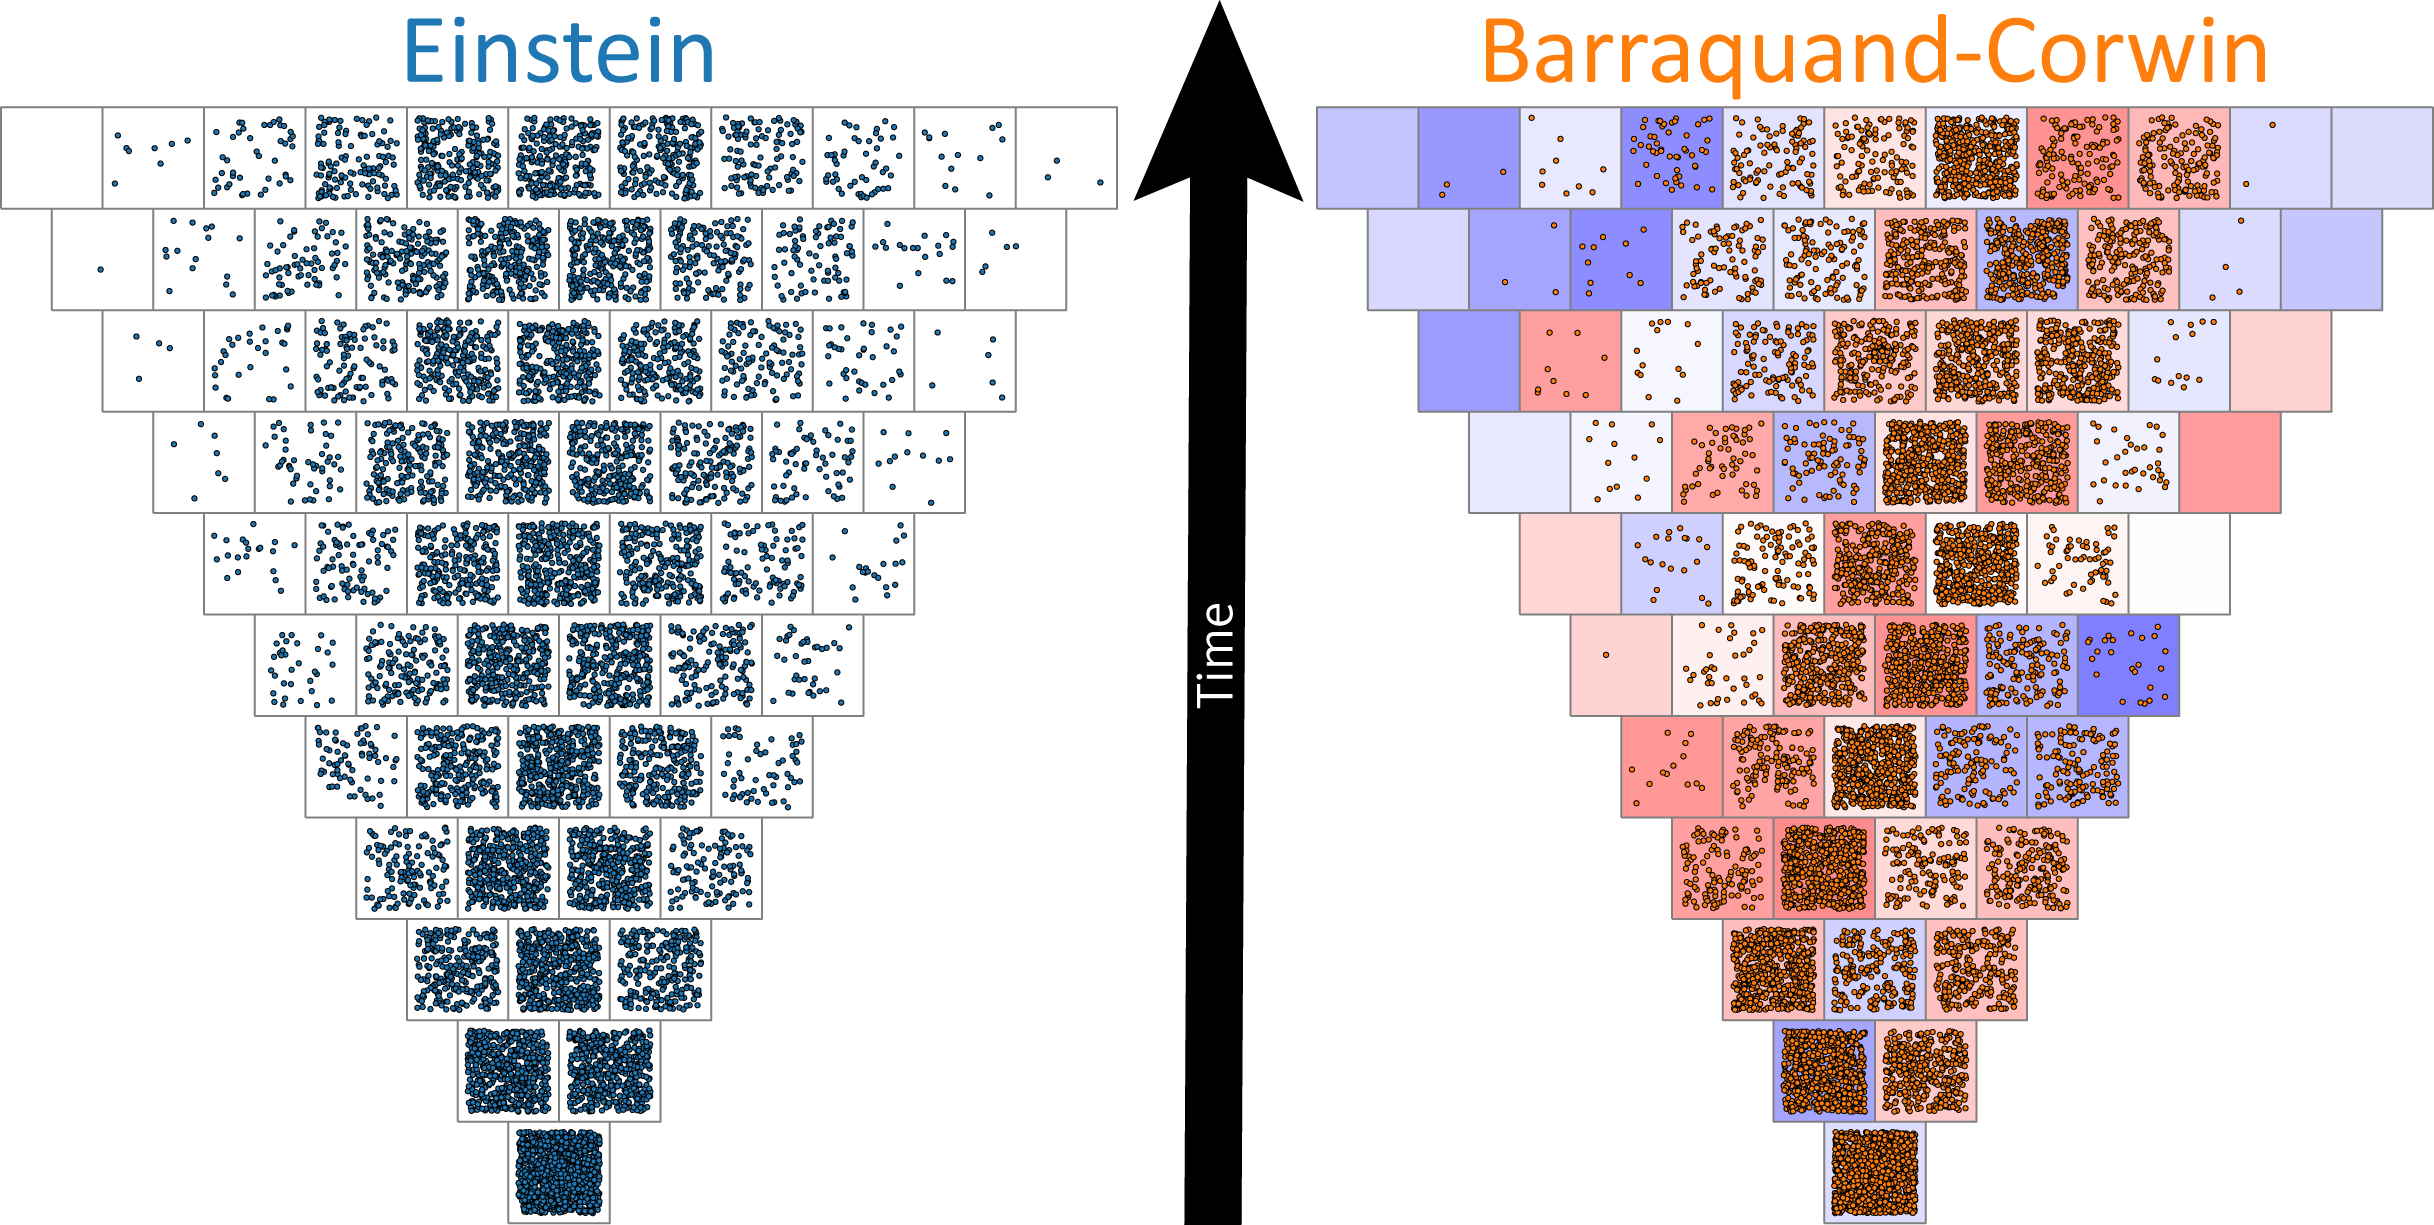
\includegraphics[width=0.9\columnwidth]{Figures/TriangleGrowth-01.png}
\caption{\label{fig:comparison} Einstein and Barraquand-Corwin diffusion models. Einstein's diffusion model has an equal bias in each direction, and the particles diffuse accordingly. For the Barraquand-Corwin model, the red and blue colors and color intensity indicate the direction and strength of the bias as in Figure \ref{fig:1D_BC}. Time increases from the bottom of the image toward the top. There is a noticeable difference in how the outlier particles for each model spread in the same amount of time.}
\end{center}
\end{figure*}

The first known observations of irregular, wiggly movements characteristic of small particles may be attributed to the work of Jan Ingenhousz, who described the motion of coal dust on the surface of alcohol in 1785~\cite{ingenhousz_new_1785}. In the following century, while scientists worked to theoretically understand and mathematically describe the processes by which all sorts of stuff spreads out, Robert Brown published observations of the seemingly random motion of diffusive particles, like the dust that floats through air and the motion of pollen on the surface of water~\cite{brown_xxvii_1828,brown_xxiv_1829,van_der_pas_discovery_1971}. Brown's descriptions of this motion became quite prolific, and the name ``Brownian motion'' caught on. Connecting diffusion models with Brownian motion observations was built upon the ``random walk'' concept, proposed in Jules Regnault's 1863 publication and Louis Bachelier's 1900 thesis, both of which described small price changes in stock market shares as random and unpredictable ``steps'' in an overall ``walk''~\cite{regnault_calcul_1863,bachelier_theorie_1900}. In 1905, Einstein used a random walk model to formulate a diffusion equation to describe Brownian motion, with a diffusion coefficient controlling the step size~\cite{einstein_uber_1905}. Marian von Smoluchowski and William Sutherland both independently, concurrently characterized Brownian motion in the same manner~\cite{sutherland_lxxv_1905,von_smoluchowski_zur_1906}. 

The random walk model for diffusion proposed that the visible particles exhibiting the characteristic wiggly Brownian motion are moving through an invisible environment of molecules, which are constantly moving around because of their inherent thermal energy. These molecules collide with the larger visible particles, pushing them around from all sides and causing their apparent erratic motion. This motion causes the diffusing particles to undergo a random walk with independent random ``steps’’, changing the particle's location throughout time. This distribution of steps has a variance controlled by a diffusion coefficient, which is dependent on both the diffusing particle and the environment. Einstein derived the Brownian motion random walk model through the molecular-kinetic theory of heat, connecting it to the differential equation Fick had developed decades before, and relating the diffusion coefficient to many physical quantities which can be measured~\cite{einstein_uber_1905}. Experimentalists Jean Baptiste Perrin and Christina Cruickshank Miller confirmed the validity of Einstein's, Sutherland's, and Smoluchowski's work~\cite{perrin_mouvement_1909,cruickshank_miller_stokes-einstein_1924}. The random walk model results, from the diffusion differential equation to the Stokes-Einstein-Sutherland relation, can be used to understand many processes dominated by diffusion of the bulk of the material very well. The ability to describe the average diffusing particle and predict statistical behavior has led to all sorts of insight into a wide variety of important physical systems.
% , in applications including a broad range of biological and chemical processes~\cite{kao_virus_2006,le_bihan_mr_1986,le_bihan_diffusion_2014,abdel_razek_apparent_2019,sykova_diffusion_2008,nicholson_extracellular_1998,nicholson_diffusion_2001,wijman_prognostic_2009} and genetics~\cite{feller_diffusion_1951,wakeley_limits_2005,ewens_mathematical_2012,waxman_diffusion_2017}.


While the random walk model of diffusion has worked very well to describe the average particle, there are many instances in which this model fails, whether from active matter injecting energy into the system or because the diffusion coefficient varies in space or time.
% ~\cite{wang_when_2012,kanazawa_loopy_2020,bouchaud_anomalous_1990,ghosh_non-universal_2015,metzler_brownian_2019,das_non-fickian_1998}.
A strong explanation for this failure is that the random walk model described by Einstein requires each particle to take a totally independent path relative to every other particles, including those nearby, which we would expect to be influenced by their shared environment in similar ways.
The failure of this model is especially evident in the statistical behavior of the extreme particles, the ones that travel the furthest distance from the origin or which cross a certain distance first, which are critical in many applications that rely on the first particle to travel from the origin to a specific distance or target.
% including stock market fluctuations~\cite{barney_first-passage-time_2017,liu_anchoring_2017} chemical reactions and channel transport~\cite{redner_guide_2001,iyer-biswas_first_2015}, fertilization~\cite{grebenkov_escape_2017,grebenkov_molecular_2021}, protein dynamics~\cite{polizzi_mean_2016} and menopause timing~\cite{lawley_slowest_2023}. 
To account for background correlations, one could instead require that particles undergo a random walk in a random environment, where the probability that a particle will ``step'' in a given direction varies in space and time. Such an environment can be seen in Figure \ref{fig:1D_BC}, contrasted with that of the ``Einstein'' uncorrelated random walk. 
% Mathematical work has proposed alternate models to account for anomalous diffusion, from the random walk in a random environment~\cite{barraquand_random-walk_2017,le_doussal_diffusion_2017} to random walks in fractal media~\cite{hentschel_relative_1984,chun_heterogeneous_2023,condamin_first-passage_2007} and countless others~\cite{condamin_first-passage_2007,havlin_diffusion_2002,barraquand_moderate_2020}.
As seen in Figure \ref{fig:comparison}, while the bulk of the diffusing particles doesn't vary between the models, the behavior of the particles furthest from the origin varies. The behavior in the correlated environment is more ``sticky'' -- particles close together stick together, following the stronger biases. We expect the outlier particles to be characterized by different statistics than the average~\cite{lawley_distribution_2020,lawley_probabilistic_2020,lawley_universal_2020}, and we  anticipate the emergence of different scaling regimes based on the introduced spatial and temporal biases~\cite{barraquand_random-walk_2017,le_doussal_diffusion_2017}.

% What do we see when we observe systems undergoing diffusion, both numerically and physically? For the first part of my graduate career, I explored this question through the random walk in a random environment theoretical framework. I consider a random walk in an environment that is correlated rather than totally independent, by using a spatially and temporally varying bias field to influence particles close together to behave similarly to each other. In this dissertation I show that the introduction of this field in numerical simulations allows us to explore the resulting statistical descriptions, and I find that we can actually tease out information about the shared environment from the measurements of the diffusing particles. Additionally, I can use micron-sized silica beads suspended in water, which display the same thermal motions that Brown observed in pollen grains almost 200 years ago, to measure the extreme statistics in a real physical system. I demonstrate proof of concept of such an experiment.

Additionally, photons sent into random media scatter in a way that appears analogous to random-walk-model diffusion. With relatively high scatterer concentration and minimal absorption, we can use a diffusion approximation to the nontrivial Boltzmann Radiative Transfer Equation to model photon propagation~\cite{ishimaru_wave_1997}. This approximation neglects the speed of light in a medium, and as a result, it accurately describes the average photon within the bounds of the approximation but fails outside of these bounds.
% The diffusion approximation predicts the behavior of the average photon travelling through random media well, and offers valuable insights into systems in many applications~\cite{haskell_boundary_1994,  chandrasekhar_stochastic_1943,chandrasekhar_radiative_1950,  brown_light_1975, allgaier_diffuse_2021, taitelbaum_diagnosis_1999, amendola_accuracy_2021}. 
% However, by neglecting that photons travel at the speed of light in a medium, this model fails at short length and time scales, media with significant anisotropy or absorption, or environments with low scattering~\cite{ishimaru_wave_1997, yoo_time-resolved_1990, yoo_when_1990, durian_photon_1997, zhang_wave_2002, pierrat_photon_2006}. 
By retaining a second-order time derivative in the diffusion approximation, or by accounting for photons as two opposing ``streams'', we can find a telegraph equation model that factors in this constant speed of light and overcomes many of the diffusion approximation limitations~\cite{lemieux_diffusing-light_1998}.
% A telegraph equation model overcomes many of these limitations by accounting for ballistic photons and wave-like effects present at small distances, leading to more accurate predictions of photon behaviors~\cite{goldstein_diffusion_1951, durian_two-stream_1996, durian_photon_1997, lemieux_diffusing-light_1998, masoliver_solutions_1992, masoliver_finite-velocity_1996, das_non-fickian_1998, polishchuk_photon-density_1997}. Discrepancies remain at distances relatively close to the source~\cite{durian_photon_1997, dudko_photon_2005, lemieux_diffusing-light_1998}, and the accuracy of the predicted speed of light depends on how scattering properties are approximated during the derivation~\cite{heizler_asymptotic_2012, hoenders_telegraphers_2005, polishchuk_photon-density_1997}.
Both models have described the average photon well, and photon propagation in scattering media has been characterized and used in a broad range of applications. However, the extreme value statistics of photons in scattering media have not been measured, and could reveal the limits of the uncorrelated random walk model that underlies both of these approximations to the radiative transfer equation.


% In photonic systems, changes in pulse shape due to absorption and scattering have been measured~\cite{lee_using_2007,madsen_experimental_1992,ishimaru_diffusion_1978,yoo_time-resolved_1990,yoo_when_1990,zhang_wave_2002,calba_ultrashort_2008}, and photon first passage time distributions have been characterized numerically and experimentally~\cite{rossetto_isotropic_2022,long_particle_2001,weiss_applications_2002,zeller_light_2020}. To our knowledge, photon extreme first passage time distributions have not previously been experimentally measured. 

% The remainder of my graduate work has centered on this phenomenon, with the goal of measuring these extreme first passage times and determining how the distribution changes as the scattering properties of the medium change. The diffusion approximation always fails to describe extreme first passage photons because it ignores the speed of light, and the telegraph equation predicts extreme photons that travel directly through an index-averaged medium until a certain concentration at which the predicted times diverge and increase rapidly with scatterer concentration. Extreme first passage time distributions I measured show that the extreme photons travel directly through the medium without scattering around, even long after the predictions expect a divergence, revealing flaws in the underlying assumption that photon paths are independent from each other.

The following chapters are a coauthored paper, unpublished work, and a first author paper, all of which I composed during my time as a graduate student. Chapter \ref{ch2_1Drandom} (published in PRE~\cite{hass_anomalous_2023}) explores a method that I developed along with Eric Corwin and Jacob Hass. This allowed us to numerically simulate diffusion systems, and measure the location of the farthest particle from the origin, and I uncovered a new phase with connections to the Kardar-Parisi-Zhang universality class. In chapter \ref{ch3_extras}, I developed an experimental apparatus that doubles as a centrifuge and a microscope stage in order to observe diffusion in colloidal suspensions, and I report on current design and the potential for future work, particularly in using this experiment to verify results found in Chapter \ref{ch2_1Drandom} and additional work on extreme first passage times~\cite{hass_first-passage_2024}. In Chapter \ref{ch4_photons} (in review,~\cite{carroll-godfrey_measurements_2025}), I used an ultrafast pulsed laser to send bursts of photons into a tube filled with silica nanospheres, timing the first photon to exit the tube, and build histograms of extreme first passage times. I measured the peak of this distribution, and determined that neither the diffusion nor telegraph model for photon transport correctly predicts the peak location; correlations cause more photons to travel directly through the tube as though they see an index-averaged medium.